\section{Functionality}

\todo{thomas, read this}
\autoref{fig:design_diagram} shows the states divided into functionality groups, which describe a specific feature from the backlog.

%To specificy a more detailed design, the need for narrowing down the abstract states into features are required.
%The states are divided into feature groups, which can seen in \autoref{fig:design_diagram}.
%Each feature's functionality is defined by each outgoing action from the states the feature originates from. 

\begin{figure}[h]
	\centering
	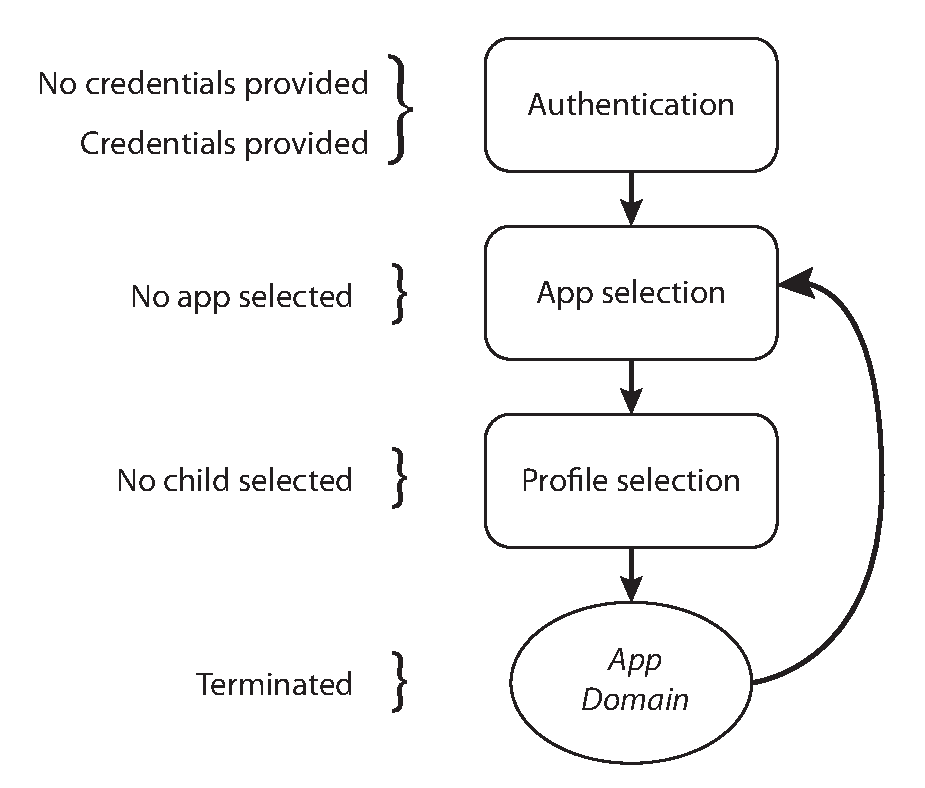
\includegraphics[width=1\textwidth]{gfx/design_diagram.pdf}
	\caption{Design diagram}
	\label{fig:design_diagram}
\end{figure}
\todo{Wombat og Parrot skal skrives med stort}

\subsection{Authentication}


\noindent The authentication consists of two steps:

\begin{enumerate}
	\item validating
	\item confirmation
\end{enumerate}

The validation step consists of scanning the provided QR-code. If valid, the user is asked to confirm the scanned identity, or reject if needed. The user is not allowed to proceed if the QR-code is unvalid.

Confirmation is chosen, in order to avoid authentications where a user uses a QR-code which is not the one the user thought it was.

%Upon scanning a QR-code, there is two possible outcomes: The QR-code is invalid, as the credentials are not recognized, or the QR-code contains credentials which are recognized.
%In case of the QR-code being valid, the process then enters it second step. The second step consist of the user needs to confirm the identity, or reject if identity represented on the system does not match the user's identity. 

\subsection{App management}
\label{design:app_manangement}
The app management functionality is illustrated in \autoref{fig:appmanagement_design}. 
\begin{figure}[h]
	\centering
	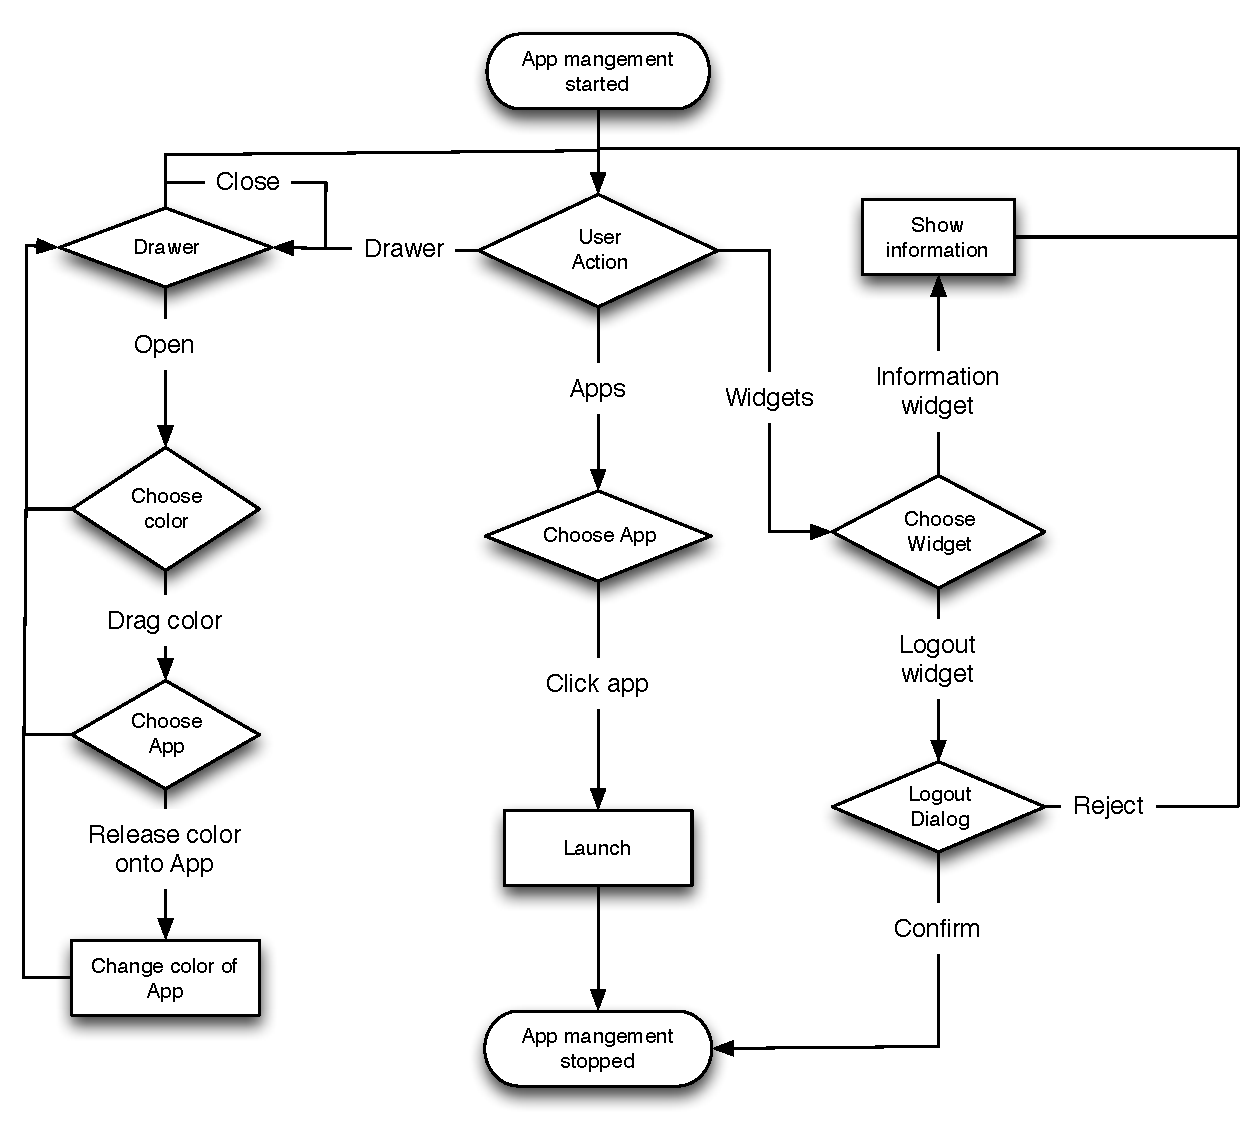
\includegraphics[width=1\textwidth]{gfx/appmanagement.pdf}
	\caption{Features of the App management feature}
	\label{fig:appmanagement_design}
\end{figure}
User interaction is the initial step of the app management functionality, and can be one of the three interactions:

\begin{enumerate}
	\item Change app settings
	\item Launch app
	\item Request information
\end{enumerate}

%User action is the initial step of the app management feature, and controls the interaction with the user.
%One of the actions the user is able to make, is to change settings regarding the current authenticated user's apps.
The user does that by interacting with the drawer \todo{insert ref to preanalysis}.
The drawer can be opened or closed.
The closed state is when the drawer is sled all the way to the left.
The open state is when the drawer is when is not sled all the way to the left, and is below or at its maximum span.
When the drawer is opened, it is possible to change a color of an app.
This is done by dragging a color from the color table, onto an app and releasing in order to make the app change color.
The system can then return to the initial state.

Another action the user is able to make, is to retrieve information regarding the system.
After the information have been shown to the user, the user returns to the initial state.
The last action the user is able to make from the initial state is to launch an app.
This is done by the user clicking on the app, and then app management process is over.

\subsection{Profile selection}
The profile selection feature is illustrated in \autoref{fig:profileselection_design}. 
\label{design:profile_selection}
\begin{figure}[h]
	\centering
	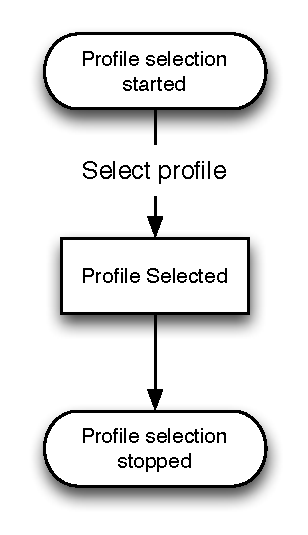
\includegraphics[width=0.3\textwidth]{gfx/profileselect_design.pdf}
	\caption{Features of the Profile selection feature}
	\label{fig:profileselection_design}
\end{figure}
The initial state of this feature is to choose which profile the previous selected should be launched as. This done by clicking on the chosen profile. If the chosen profile is not visible on the screen, it can be needed to scroll through the profiles in order to find it. When the chosen is clicked, the profile is selected and the profile selection process is over.